
\documentclass[12pt]{article}
\usepackage{amsmath}
\usepackage{geometry}
\usepackage{graphicx}
\usepackage{array}
\usepackage{longtable}
\usepackage{hyperref}
\geometry{margin=1in}

\title{CSC6033 - Week 6 Coding Project (P\#6)\\Turing Machine for Unary Addition}
\author{Irfan Ahmed}
\date{}

\begin{document}
\maketitle

\section*{Unary Number Representation}
In unary notation:
\begin{itemize}
    \item A number $n$ is represented by $n$ occurrences of the symbol \texttt{0}.
    \item Two numbers are separated by a special symbol, e.g., \texttt{\#}.
\end{itemize}

\textbf{Examples:}
\begin{itemize}
    \item $2 \rightarrow$ \texttt{00}
    \item $3 \rightarrow$ \texttt{000}
    \item $2 + 3 \rightarrow$ \texttt{00\#000} $\Rightarrow$ Result: \texttt{00000}
\end{itemize}

\section*{Objective}
Design a Turing Machine (TM) that:
\begin{itemize}
    \item Accepts two unary numbers separated by \texttt{\#}
    \item Replaces \texttt{\#} with \texttt{0} to merge the two sequences
    \item Replaces the last \texttt{0} with a blank (\texttt{B}) to mark the end
    \item Halts after completing the addition
\end{itemize}

\section*{Formal Definition of the Turing Machine}
\textbf{M = (Q, $\Sigma$, $\Gamma$, $\delta$, $q_0$, B, F)}

\begin{itemize}
    \item $Q = \{q_0, q_1, q_2, q_3\}$ \hfill (Set of states)
    \item $\Sigma = \{0, \#\}$ \hfill (Input alphabet)
    \item $\Gamma = \{0, \#, B\}$ \hfill (Tape alphabet)
    \item $\delta$ = Transition function
    \item $q_0$ = Start state
    \item $B$ = Blank symbol
    \item $F = \{q_3\}$ \hfill (Final state)
\end{itemize}

\section*{Transition Table}
\begin{longtable}{|c|c|c|c|c|}
\hline
\textbf{Current State} & \textbf{Read Symbol} & \textbf{Write Symbol} & \textbf{Move} & \textbf{Next State} \\
\hline
$q_0$ & 0 & 0 & R & $q_0$ \\
$q_0$ & \# & 0 & R & $q_1$ \\
$q_1$ & 0 & 0 & R & $q_1$ \\
$q_1$ & B & B & L & $q_2$ \\
$q_2$ & 0 & B & N & $q_3$ (halt) \\
\hline
\end{longtable}

\section*{State Diagram}
\begin{figure}[h!]
\centering
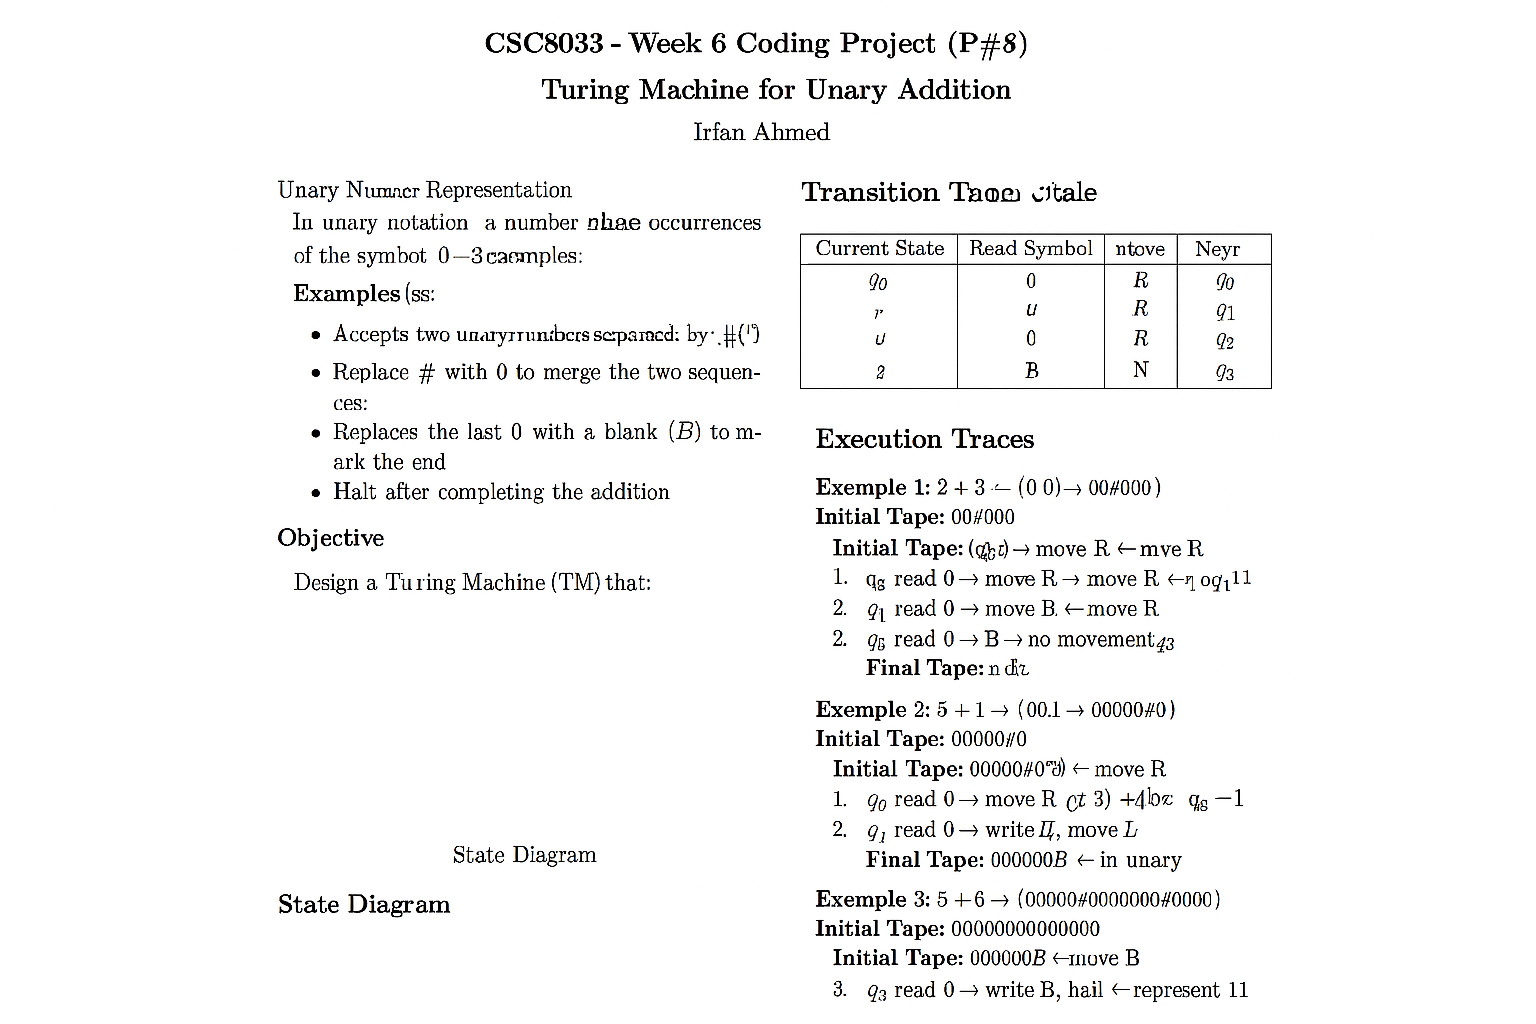
\includegraphics[width=0.8\textwidth]{state_diagram.png}
\caption{State Diagram of the Turing Machine for Unary Addition}
\end{figure}

\section*{Execution Traces}

\subsection*{Example 1: $2 + 3 \rightarrow$ \texttt{00\#000}}
\textbf{Initial Tape:} \texttt{00\#000}

\textbf{Steps:}
\begin{enumerate}
    \item $q_0$, read 0 $\rightarrow$ move R
    \item $q_0$, read 0 $\rightarrow$ move R
    \item $q_0$, read \# $\rightarrow$ write 0, move R $\rightarrow q_1$
    \item $q_1$, read 0 $\rightarrow$ move R
    \item $q_1$, read 0 $\rightarrow$ move R
    \item $q_1$, read 0 $\rightarrow$ move R
    \item $q_1$, read B $\rightarrow$ move L $\rightarrow q_2$
    \item $q_2$, read 0 $\rightarrow$ write B, halt $\rightarrow q_3$
\end{enumerate}

\textbf{Final Tape:} \texttt{000000B} $\Rightarrow$ represents 5 in unary

\subsection*{Example 2: $5 + 1 \rightarrow$ \texttt{00000\#0}}
\textbf{Initial Tape:} \texttt{00000\#0}

\textbf{Steps:}
\begin{enumerate}
    \item $q_0$, read 0 $\rightarrow$ move R (×5)
    \item $q_0$, read \# $\rightarrow$ write 0, move R $\rightarrow q_1$
    \item $q_1$, read 0 $\rightarrow$ move R
    \item $q_1$, read B $\rightarrow$ move L $\rightarrow q_2$
    \item $q_2$, read 0 $\rightarrow$ write B, halt $\rightarrow q_3$
\end{enumerate}

\textbf{Final Tape:} \texttt{000000B} $\Rightarrow$ represents 6 in unary

\subsection*{Example 3: $5 + 6 \rightarrow$ \texttt{00000\#000000}}
\textbf{Initial Tape:} \texttt{00000\#000000}

\textbf{Steps:}
\begin{enumerate}
    \item $q_0$, read 0 $\rightarrow$ move R (×5)
    \item $q_0$, read \# $\rightarrow$ write 0, move R $\rightarrow q_1$
    \item $q_1$, read 0 $\rightarrow$ move R (×6)
    \item $q_1$, read B $\rightarrow$ move L $\rightarrow q_2$
    \item $q_2$, read 0 $\rightarrow$ write B, halt $\rightarrow q_3$
\end{enumerate}

\textbf{Final Tape:} \texttt{00000000000B} $\Rightarrow$ represents 11 in unary

\end{document}
